

%% AAPT Physics Olympiad F=ma Questions
%%----------------------------------------


%% PhysicsOlympiad 2015
%%----------------------------------------


%% PhysicsOlympiad 1999
%%----------------------------------------
\element{aapt}{ %% Olympiad-B3
\begin{question}{olympiad-1999-q19}
    Two wave sources, $G$ and $H$, produce waves of different wavelengths as shown in the diagram.
    \begin{center}
    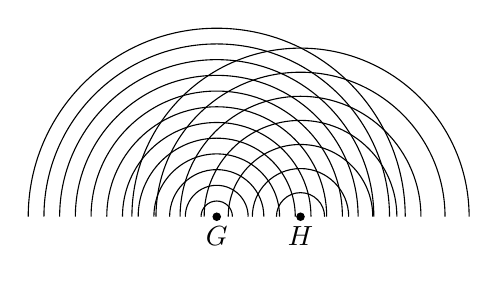
\begin{tikzpicture}[scale=1.33]
        \foreach \i in {1.5,3.0,...,18} {
            \draw (-4 mm,0) ++(\i mm,0) arc(0:180:\i mm);
        }
        \foreach \i in {2.3,4.6,...,18.4} {
            \draw (+4 mm,0) ++(\i mm,0) arc(0:180:\i mm);
        }
        \draw[fill] (-4 mm,0) circle (1pt) node[anchor=north] {$G$};
        \draw[fill] (+4 mm,0) circle (1pt) node[anchor=north] {$H$};
    \end{tikzpicture}
    \end{center}
    Lines shown in the diagram represent wave crests.
    Which of the following would be true of the resulting interference pattern?
    \begin{choices}
        \wrongchoice{The perpendicular bisector of $GH$ would be an antinodal line.}
        \wrongchoice{The interference pattern will be a stable pattern but not symmetrical left to right.}
      \correctchoice{The pattern of nodal and antinodal lines will sweep from left to right.}
        \wrongchoice{If $G$ and $H$ were moved farther apart, the fewer the number of nodal and antinodal lines.}
        \wrongchoice{There will not be an organized interference pattern because the sources are not producing the same frequency}
    \end{choices}
\end{question}
}


%% PhysicsOlympiad 1998
%%----------------------------------------
\element{aapt}{ %% Olympiad-B3
\begin{question}{olympiad-1998-q22}
    Waves are produced by two point sources $S$ and $S^{\prime}$ vibrating in phase.
    See the accompanying diagram.
    \begin{center}
    \begin{tikzpicture}
        %% Points
        \draw[fill] (-3,0) circle (2pt) node[anchor=east] {$S$};
        \draw[fill] (0,0) circle (2pt) node[anchor=east] {$S^{\prime}$};
        \draw[fill] (0,3) circle (2pt) node[anchor=east] {$X$};
        %% connect
        \draw[thick] (0,0) -- (0,3);
    \end{tikzpicture}
    \end{center}
    $X$ is a point on the second nodal line.
    The path difference $SX - S^{\prime}X$ is \SI{4.5}{\centi\meter}.
    The wavelength of the waves is approximately:
    \begin{multicols}{3}
    \begin{choices}
        \wrongchoice{\SI{1.5}{\centi\meter}}
        \wrongchoice{\SI{1.8}{\centi\meter}}
        \wrongchoice{\SI{2.3}{\centi\meter}}
      \correctchoice{\SI{3.0}{\centi\meter}}
        \wrongchoice{\SI{4.5}{\centi\meter}}
    \end{choices}
    \end{multicols}
\end{question}
}

\element{aapt}{ %% Olympiad-B3
\begin{question}{olympiad-1998-q23}
    A thin film of thickness $t$ and index of refraction 1.33 coats a glass with index of refraction 1.50 as shown below.
    \begin{center}
    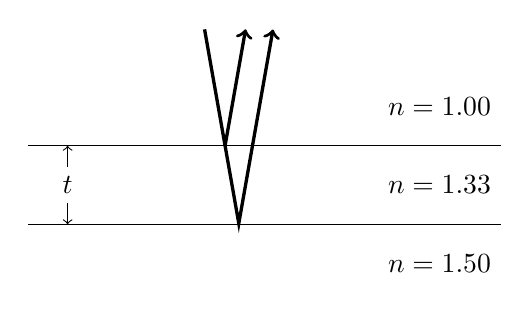
\begin{tikzpicture}
        \draw (-3,1) -- (3,1);
        \draw (-3,0) -- (3,0);
        %% thickness
        \draw[<->] (-2.5,1) -- (-2.5,0) node[pos=0.5,anchor=center,fill=white] {$t$};
        %% index of refraction
        \node[anchor=east] at (3,1.5) {$n=1.00$};
        \node[anchor=east] at (3,0.5) {$n=1.33$};
        \node[anchor=east] at (3,-0.5) {$n=1.50$};
        %% Path
        \draw[very thick] (-0.5,1) -- ++(100:1.5);
        \draw[very thick,->] (-0.5,1) -- ++(80:1.5);
        \draw[very thick,->] (-0.5,1) -- ++(-80:1.003) -- ++(80:2.5);
    \end{tikzpicture}
    \end{center}
    Which of the following thicknesses $t$ will not reflect light with wavelength \SI{640}{\nano\meter} in air?
    Hint: Light undergoes a \ang{180} phase shift when it is reflected off a material with a higher index of refraction.
    \begin{multicols}{3}
    \begin{choices}
        \wrongchoice{\SI{160}{\nano\meter}}
        \wrongchoice{\SI{240}{\nano\meter}}
      \correctchoice{\SI{360}{\nano\meter}}
        \wrongchoice{\SI{480}{\nano\meter}}
        \wrongchoice{\SI{640}{\nano\meter}}
    \end{choices}
    \end{multicols}
\end{question}
}


%% PhysicsOlympiad 1997
%%----------------------------------------
\element{aapt}{ %% Olympiad-B3
\begin{question}{olympiad-1997-q19}
    Two sources, in phase and a distance $d$ apart,
        each emit a wave of wavelength $\lambda$.
    %See accompanying figure.
    \begin{center}
    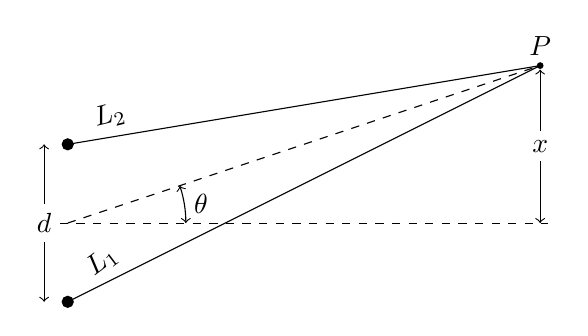
\begin{tikzpicture}
        %% Two sources
        \draw[fill] (0,+1) circle (2pt);
        \draw[fill] (0,-1) circle (2pt);
        \draw[<->] (-0.3,-1) -- (-0.3,+1) node[pos=0.5,anchor=center,fill=white] {$d$};
        %% point P
        \draw[fill] (6,2) circle (1pt) node[anchor=south] {$P$};
        \draw (0,+1) -- (6,2) node[pos=0.1,anchor=south,rotate=14] {$L_2$};
        \draw (0,-1) -- (6,2) node[pos=0.1,anchor=south,rotate=37] {$L_1$};
        %% distance x
        \draw[<->] (6,0) -- (6,1.95) node[pos=0.5,anchor=center,fill=white] {$x$};
        \draw[dashed] (-0.1,0) -- (6.1,0);
        \draw[dashed] (0,0) -- (6,2);
        \draw[<->] (1.5,0) arc (0:18.4:1.5) node[pos=0.5,anchor=west] {$\theta$};
    \end{tikzpicture}
    \end{center}
    Which of the choices for the path difference $\Delta L = L_1 - L_2$ will \emph{always} produce destructive interference at point $P$?
    \begin{multicols}{3}
    \begin{choices}
        \wrongchoice{$d\sin\theta$}
        \wrongchoice{$\dfrac{x}{L_1}$}
        \wrongchoice{$d\dfrac{x}{L_2}$}
      \correctchoice{$\dfrac{\lambda}{2}$}
        \wrongchoice{$2\lambda$}
    \end{choices}
    \end{multicols}
\end{question}
}


%% PhysicsOlympiad 1996
%%----------------------------------------
\element{aapt}{ %% Olympiad-B3
\begin{question}{olympiad-1996-q22}
    A thin film of thickness $t$ and index of refraction 1.33 coats a glass with index of refraction 1.50. 
    \begin{center}
    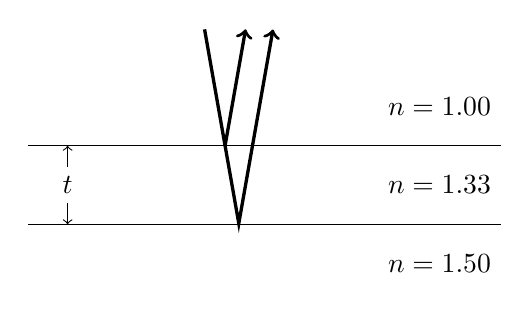
\begin{tikzpicture}
        \draw (-3,1) -- (3,1);
        \draw (-3,0) -- (3,0);
        %% thickness
        \draw[<->] (-2.5,1) -- (-2.5,0) node[pos=0.5,anchor=center,fill=white] {$t$};
        %% index of refraction
        \node[anchor=east] at (3,1.5) {$n=1.00$};
        \node[anchor=east] at (3,0.5) {$n=1.33$};
        \node[anchor=east] at (3,-0.5) {$n=1.50$};
        %% Path
        \draw[very thick] (-0.5,1) -- ++(100:1.5);
        \draw[very thick,->] (-0.5,1) -- ++(80:1.5);
        \draw[very thick,->] (-0.5,1) -- ++(-80:1.003) -- ++(80:2.5);
    \end{tikzpicture}
    \end{center}
    What is the least thickness $t$ that will strongly reflect light with wavelength \SI{600}{\nano\meter}? 
    Hint: Light undergoes a \ang{180} phase shift when it is reflected off a material with a higher index of refraction.
    \begin{multicols}{3}
    \begin{choices}
      \correctchoice{\SI{225}{\nano\meter}}
        \wrongchoice{\SI{300}{\nano\meter}}
        \wrongchoice{\SI{400}{\nano\meter}}
        \wrongchoice{\SI{450}{\nano\meter}}
        \wrongchoice{\SI{600}{\nano\meter}}
    \end{choices}
    \end{multicols}
\end{question}
}


%% PhysicsOlympiad 1995
%%----------------------------------------
\element{aapt}{ %% Olympiad-B3
\begin{question}{olympiad-1995-q22}
    Light shining through two very narrow slits produces an interference maximum at point $P$ when the entire apparatus is in air (see accompanying figure).
    \begin{center}
    \begin{tikzpicture}
        %% Two slits
        \draw[very thick] (0,-1.5) -- (0,1.5);
        \draw[white,fill=white] (0,+1) circle (4pt);
        \draw[white,fill=white] (0,-1) circle (4pt);
        \draw[<->] (-1,-1) -- (-1,+1) node[pos=0.5,anchor=center,fill=white] {$d$};
        %% point P
        \draw[fill] (6,2) circle (1pt) node[anchor=south] {$P$};
        \draw (0,+1) -- (6,2);
        \draw (0,-1) -- (6,2);
        %% distance x
        \draw[<->] (6,0) -- (6,1.95) node[pos=0.5,anchor=center,fill=white] {$x$};
        \draw[dashed] (-0.2,0) -- (6.2,0);
        \draw[dashed] (0,0) -- (6,2);
        \draw[<->] (1.5,0) arc(0:18.4:1.5) node[pos=0.5,anchor=west] {$\theta$};
    \end{tikzpicture}
    \end{center}
    For the interference maximum represented,
        light through the bottom slit travels one wavelength further than light through the top slit before reaching point $P$.
    If the entire apparatus is immersed in water,
        the angle $\theta$ to the interference maximum:
    \begin{choices}
        \wrongchoice{is unchanged}
        \wrongchoice{decreases because the frequency decreases.}
        \wrongchoice{decreases because the wavelength decreases.}
        \wrongchoice{increases because the frequency increases.}
        \wrongchoice{increases because the wavelength increases.}
    \end{choices}
\end{question}
}


%% PhysicsOlympiad 1994
%%----------------------------------------
\element{aapt}{ %% Olympiad-B3
\begin{question}{olympiad-1994-q20}
    A soap film of thickness $t$ is surrounded by air.
    It is illuminated at near normal incidence by monochromatic light which has wavelength $\lambda$ in the film.
    \begin{center}
    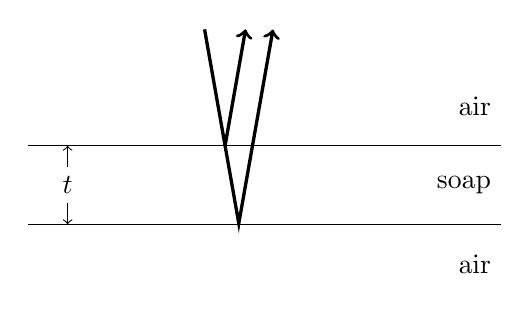
\begin{tikzpicture}
        \draw (-3,1) -- (3,1);
        \draw (-3,0) -- (3,0);
        %% thickness
        \draw[<->] (-2.5,1) -- (-2.5,0) node[pos=0.5,anchor=center,fill=white] {$t$};
        %% index of refraction
        \node[anchor=east] at (3,1.5) {air};
        \node[anchor=east] at (3,0.5) {soap};
        \node[anchor=east] at (3,-0.5) {air};
        %% Path
        \draw[very thick] (-0.5,1) -- ++(100:1.5);
        \draw[very thick,->] (-0.5,1) -- ++(80:1.5);
        \draw[very thick,->] (-0.5,1) -- ++(-80:1.003) -- ++(80:2.5);
    \end{tikzpicture}
    \end{center}
    A film thickness of \rule[-0.1pt]{4em}{0.1pt} will produce maximum brightness of the reflected light.
    \begin{multicols}{3}
    \begin{choices}
      \correctchoice{$\dfrac{\lambda}{4}$}
        \wrongchoice{$\dfrac{\lambda}{2}$}
        \wrongchoice{$\lambda$}
        \wrongchoice{$2\lambda$}
        \wrongchoice{$4\lambda$}
    \end{choices}
    \end{multicols}
\end{question}
}

\element{aapt}{ %% Olympiad-B3
\begin{question}{olympiad-1994-q23}
    Two sources, in phase and a distance $d$ apart, each emit a wave of wavelength $\lambda$.
    See accompanying figure.
    \begin{center}
    \begin{tikzpicture}
        %% Two sources
        \draw[fill] (0,+1) circle (2pt);
        \draw[fill] (0,-1) circle (2pt);
        \draw[<->] (-0.3,-1) -- (-0.3,+1) node[pos=0.5,anchor=center,fill=white] {$d$};
        %% point P
        \draw[fill] (6,2) circle (1pt) node[anchor=south] {$P$};
        \draw (0,+1) -- (6,2) node[pos=0.1,anchor=south,rotate=14] {$L_2$};
        \draw (0,-1) -- (6,2) node[pos=0.1,anchor=south,rotate=37] {$L_1$};
        %% distance x
        \draw[<->] (6,0) -- (6,1.95) node[pos=0.5,anchor=center,fill=white] {$x$};
        \draw[dashed] (-0.1,0) -- (6.1,0);
    \end{tikzpicture}
    \end{center}
    Which of the choices for the path difference $\Delta L = L_1 - L_2$ will always produce constructive interference at point $P$?
    \begin{multicols}{3}
    \begin{choices}
        \wrongchoice{$d\sin\theta$}
        \wrongchoice{$\dfrac{x}{L_1}$}
        \wrongchoice{$d\left(\dfrac{x}{L_2}\right)$}
        \wrongchoice{$\dfrac{\lambda}{d}$}
      \correctchoice{$2\lambda$}
    \end{choices}
    \end{multicols}
\end{question}
}


\endinput


